%------------------------------------------------------------------------------
% Author(s):
% Varaun Ramgoolie
% Copyright:
%  Copyright (C) 2020 Brad Bachu, Arjun Mohammed, Varaun Ramgoolie, Nicholas Sammy
%
%  This file is part of Applied-Mathematics-Unit2 and is distributed under the
%  terms of the MIT License. See the LICENSE file for details.
%
%  Description:
%     Year: 2015
%     Module: 3
%     Question: 6 
%------------------------------------------------------------------------------

%------------------------------------------------------------------------------
% 6 a
%------------------------------------------------------------------------------

\begin{subquestions}

\subquestion
We are given a situation where water hits a wall at a certain rate and does not bounce back.

\textbf{\textit{Sketch and Translate:}} \\ \\
\begin{figure}[H]
	\begin{center}
		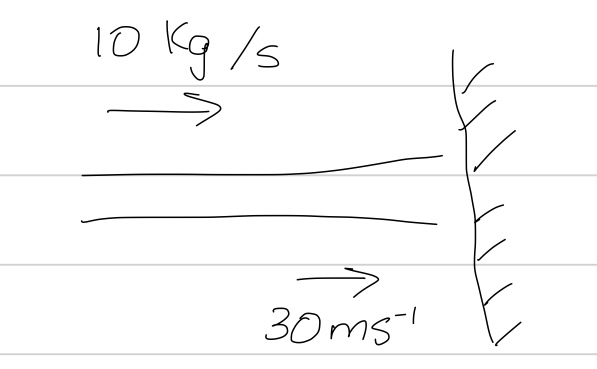
\includegraphics[scale=0.25]{../2015/figures/2015q6-1}
		\caption{\label{2015:q6:fig:Sketch1} Water hitting the wall.}
	\end{center}
\end{figure}
We want to find the average force exerted on the wall, given the flow rate of the water and the assumption that the water does not bounce off the wall. We should begin thinking about the relationships that we know with force and the speed/motion of a body.




\textbf{\textit{Simplify and Diagram:}} \\ \\
\begin{figure}[H]
	\begin{center}
		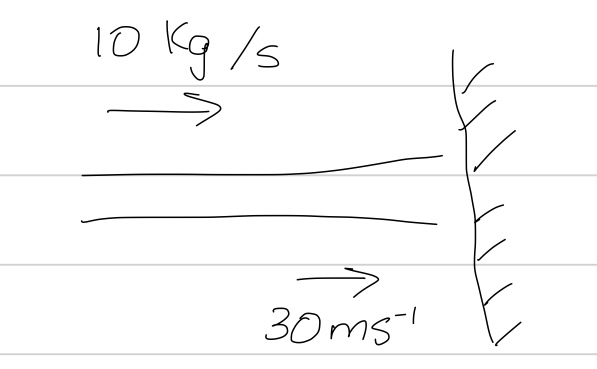
\includegraphics[scale=0.25]{../2015/figures/2015q6-1}
		\caption{\label{2015:q6:fig:Diagram1} Water hitting the wall.}
	\end{center}
\end{figure}	
As we are to assume that the water does not bounce off the wall, we can consider the final speed of the water as 0. We are given the flow rate of the water in kgs$^{-1}$ so we should think about equations of force that include a term that looks like $\frac{mass}{time}=\frac{m}{t}$. We shall consider Newton's Second Law. We will also assume that the water is moving in 1 dimension only.
	
	
	
	
\textbf{\textit{Represent Mathematically:}} \\ \\
From Newton's Second Law, we know that,
\begin{equation}
	F=ma \,.
\end{equation}
	
If we expand this, we get that,
\begin{align}
	F & = ma \nn \\
	  & = m\frac{(v-u)}{t} \nn \\
	  & = \frac{m}{t}(v-u) \,.
\end{align}
	
	
	
	
\textbf{\textit{Solve and Evaluate:}} \\ \\
Considering the moment as the water is about to hit the wall, we get that $u=30$ms$^{-1}$, $v=0$, and $\frac{m}{t}=10$kgs$^{-1}$. Substituting these values, we get that,
\begin{align}
	F & = \frac{m}{t}(v-u) \nn \\
	  & = 10(0-30) \nn \\
	  & = -300N \,.
\end{align}	
	
As force is a vector, we must be mindful that this value considers the direction from $v$ to $u$. Therefore, the true average force exerted in the direction of $u$ to $v$ is -(-300N) which is 300N.
	
%------------------------------------------------------------------------------
% 6 b
%------------------------------------------------------------------------------

\subquestion
We are given a situation where a collision occurs and the bodies become coupled after the collision.

\textbf{\textit{Sketch and Translate:}} \\ \\
\begin{figure}[H]
	\begin{center}
		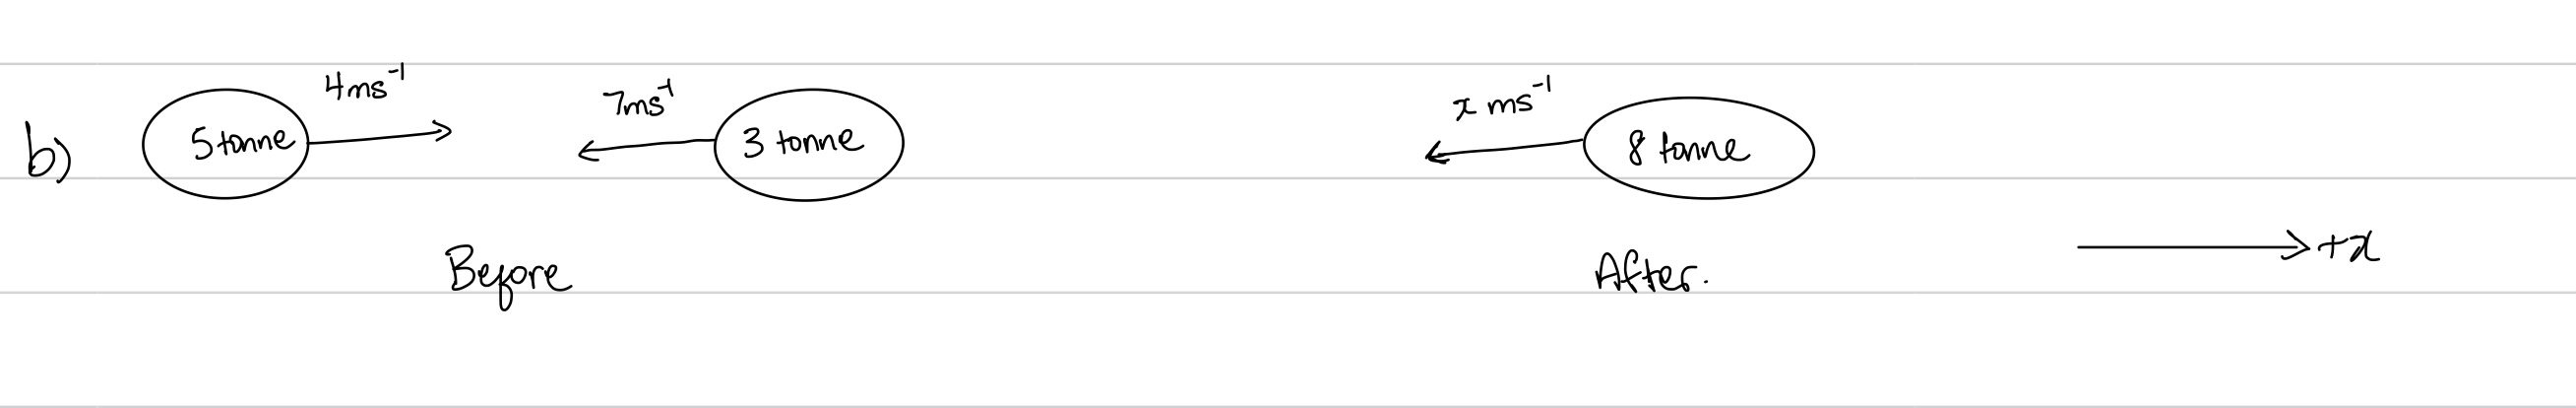
\includegraphics[scale=0.25]{../2015/figures/2015q6-2}
		\caption{\label{2015:q6:fig:Sketch2} Bodies colliding with each other.}
	\end{center}
\end{figure}	
We are asked to find the velocity and direction of the coupled body after impact. As we are given the mass and velocities of the bodies, we should begin thinking about what we know about their relationship and the momentum of the bodies.
	
	
	
	
\textbf{\textit{Simplify and Diagram:}} \\ \\
\begin{figure}[H]
	\begin{center}
		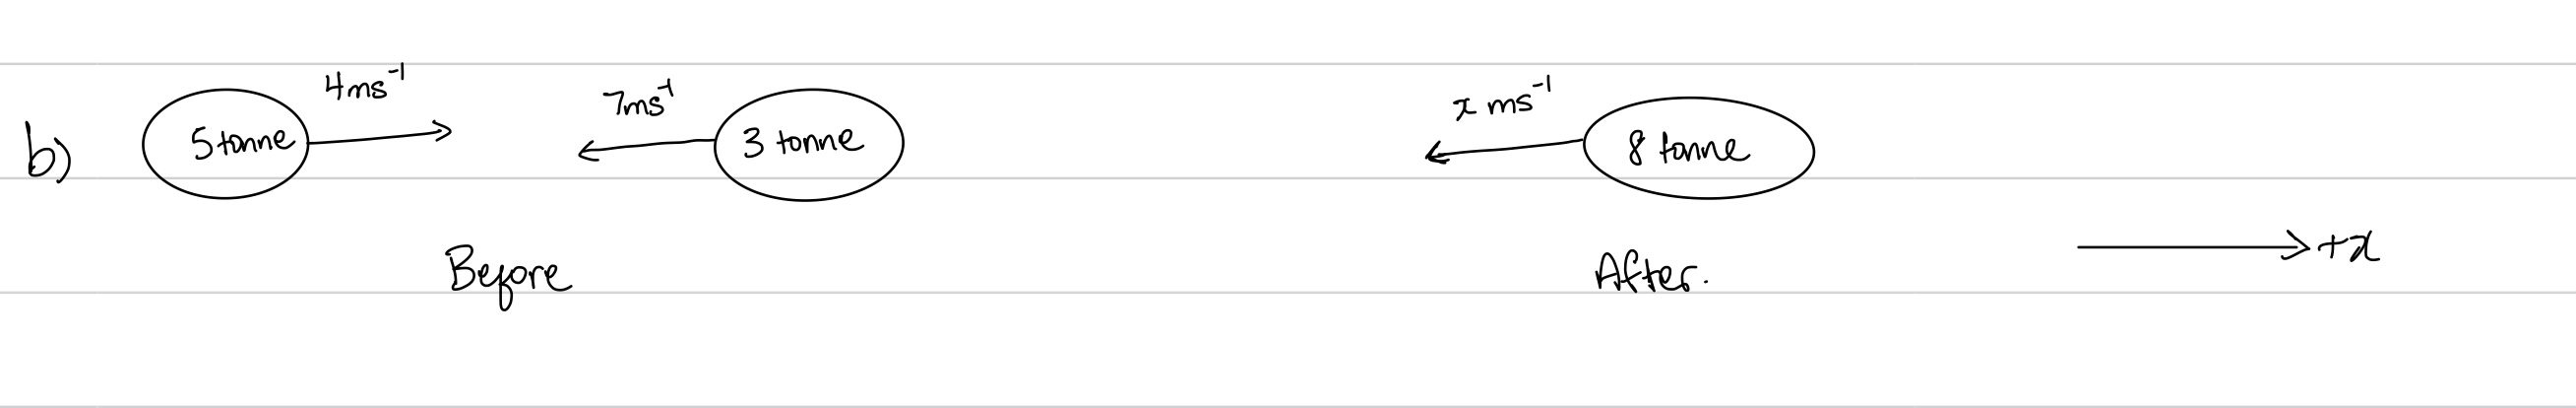
\includegraphics[scale=0.25]{../2015/figures/2015q6-2}
		\caption{\label{2015:q6:fig:Diagram2} Collision overview with velocities and masses.}
	\end{center}
\end{figure}
We will assume that the collision occurs in a closed system (no external forces acting on the system). We will take movement to the right as positive and we will assume that the bodies only move in 1 dimension. We can use the Law of Conservation of Momentum to solve this problem.




\textbf{\textit{Represent Mathematically:}} \\ \\
From the Law of Conservation of Momentum, we get that,
\begin{align}
	\text{Total Momentum Before collision} & = \text{Total Momentum After collision} \nn \\
	m_1v_1 + m_2v_2 & = (m_1+m_2)v_3 \,.
\end{align}
	
	
	
	
\textbf{\textit{Solve and Evaluate:}} \\ \\
Substituting the values of $m_1=5000$kg, $m_2=3000$kg, $v_1=4$ms$^{-1}$ and $v_2=-7$ms$^{-1}$, we get,
\begin{align}
	m_1v_1 + m_2v_2 & = (m_1+m_2)v_3 \nn \\
	5000\times4 + 3000\times-7 & = (5000+3000)v_3 \nn \\
	\implies v_3 & = \frac{20000-21000}{8000} \nn \\
	             & = \frac{-1}{8}\text{ms}^{-1}
\end{align}
The negative sign indicates that the coupled body is moving to the left (as we took the positive direction as to the right).
	
%------------------------------------------------------------------------------
% 6 c
%------------------------------------------------------------------------------

\subquestion
We are given a pulley system where two masses, are held by a light, inextensible string.

\textbf{\textit{Sketch and Translate:}} \\ \\
\begin{figure}[H]
	\begin{center}
		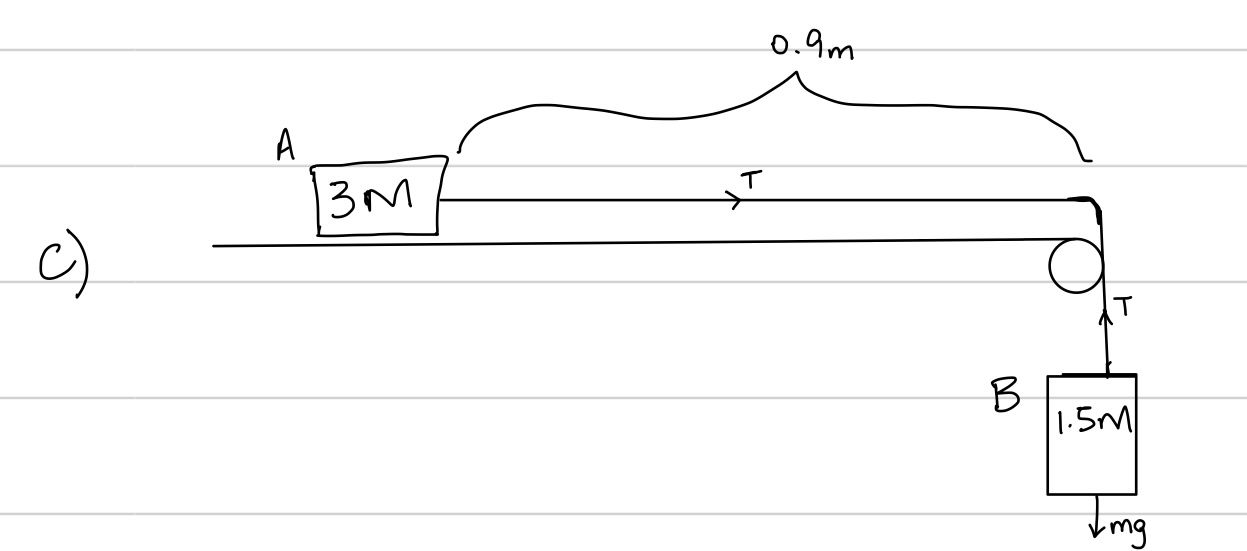
\includegraphics[scale=0.25]{../2015/figures/2015q6-3}
		\caption{\label{2015:q6:fig:Sketch3} Pulley System.}
	\end{center}
\end{figure}	
We are asked to find the speed of block A as it reaches the edge of the table. We are given the lengths and dimensions of parts of the system and we are explicitly asked to use the Principle of Conservation of Mechanical Energy. Therefore, we should begin thinking about what we know about how energy is conserved in pulley systems like these.




\textbf{\textit{Simplify and Diagram:}} \\ \\
\begin{figure}[H]
	\begin{center}
		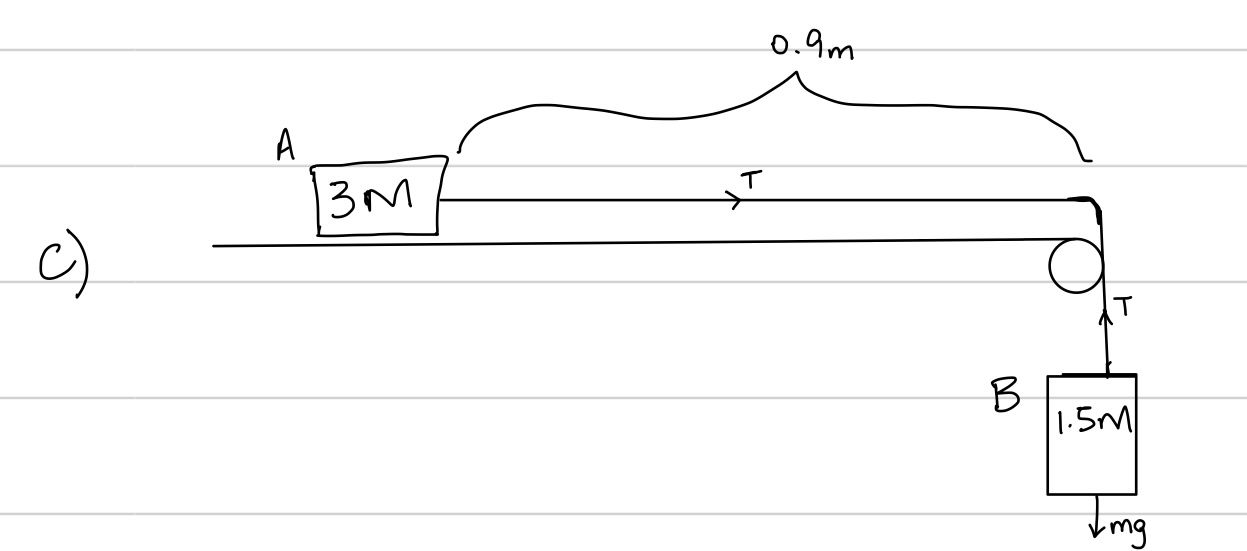
\includegraphics[scale=0.25]{../2015/figures/2015q6-3}
		\caption{\label{2015:q6:fig:Diagram3} Full layout of Pulley System.}
	\end{center}
\end{figure}
We will assume that both bodies move in separate 1 dimensional spaces only (A will move in the $x$ direction and B will move in the $y$ direction). As the string is light, we can assume that the mass of the string is 0. Similarly, as the string is inextensible, we know that the speed of both particles must be the same (but their velocities will be different due to their movement in perpendicular directions). We are also given that the system is released from rest which means that both particles possess no Initial Kinetic Energy.
	
	
	
	
\textbf{\textit{Represent Mathematically:}} \\ \\
Using the Principle of Conservation of Mechanical Energy, we know that throughout the system,
\begin{align}
	\text{Initial Kinetic Energy + Initial Potential Energy} & = \text{Final Kinetic Energy + Final Potential Energy} \nn \\
	KE_I + PE_I & = KE_F + PE_F \,. \label{2015:q6:energy1}
\end{align}

From the system, we know that B will lose PE as it is falling downwards. We can consider the initial PE as 0. We must notice that the maximum height that B can fall (while A is still on the horizontal plane) is 0.9m. Therefore, we get that the Total Final PE of the system\footnote{We can consider this as the total potential energy of the system as A does not move in the vertical plane at all. The potential energy of the system is solely dependent on B.} is,
\begin{align}
	PE_F &  = m_Bg\Delta h - 0 \nn \\
	          & = 1.5Mg(-0.9) \nn \\
	          & = -1.35Mg
\end{align}

As the string is inextensible, the speed of both particles must be the same. Therefore, we get that the Total Final KE of the system is,
\begin{align}
	KE_F & = KE_A + KE_B \nn \\
	     & = \frac{1}{2}(3M)(v^2) + \frac{1}{2}(1.5M)(v^2) \nn \\
	     & = \frac{4.5M}{2}v^2 \,.
\end{align}




\textbf{\textit{Solve and Evaluate:}} \\ \\
From the constraints given, we know that $KE_I=0$ and we can consider $PE_I$ to be 0. Substituting these into \req{2015:q6:energy1}, 
\begin{align}
	KE_I + PE_I & = KE_F + PE_F \nn \\
	0 + 0 & = \frac{4.5M}{2}v^2 - 1.35Mg \nn \\
	\frac{4.5M}{2}v^2 & = 1.35Mg \nn \\
	v^2 & = \frac{2.7g}{4.5} \nn \\
	    & = \frac{3g}{5} \nn \\
	    \implies v & = \sqrt{\frac{3g}{5}} \nn \\
	               & = \sqrt{6} \approx 2.45 \text{ms}^{-1} \,.
\end{align}

We should be mindful that this is not the only approach to this question. We can also use a Forces approach and reach the same result (See the Second Solution). However, the question explicitly asked for a Conservation of Mechanical Energy approach to solve the question.
	
%------------------------------------------------------------------------------
% 6 d
%------------------------------------------------------------------------------

\subquestion
We are given two masses which are connected by a string over a smooth, weightless pulley.

\textbf{\textit{Sketch and Translate:}} \\ \\
\begin{figure}[H]
	\begin{center}
		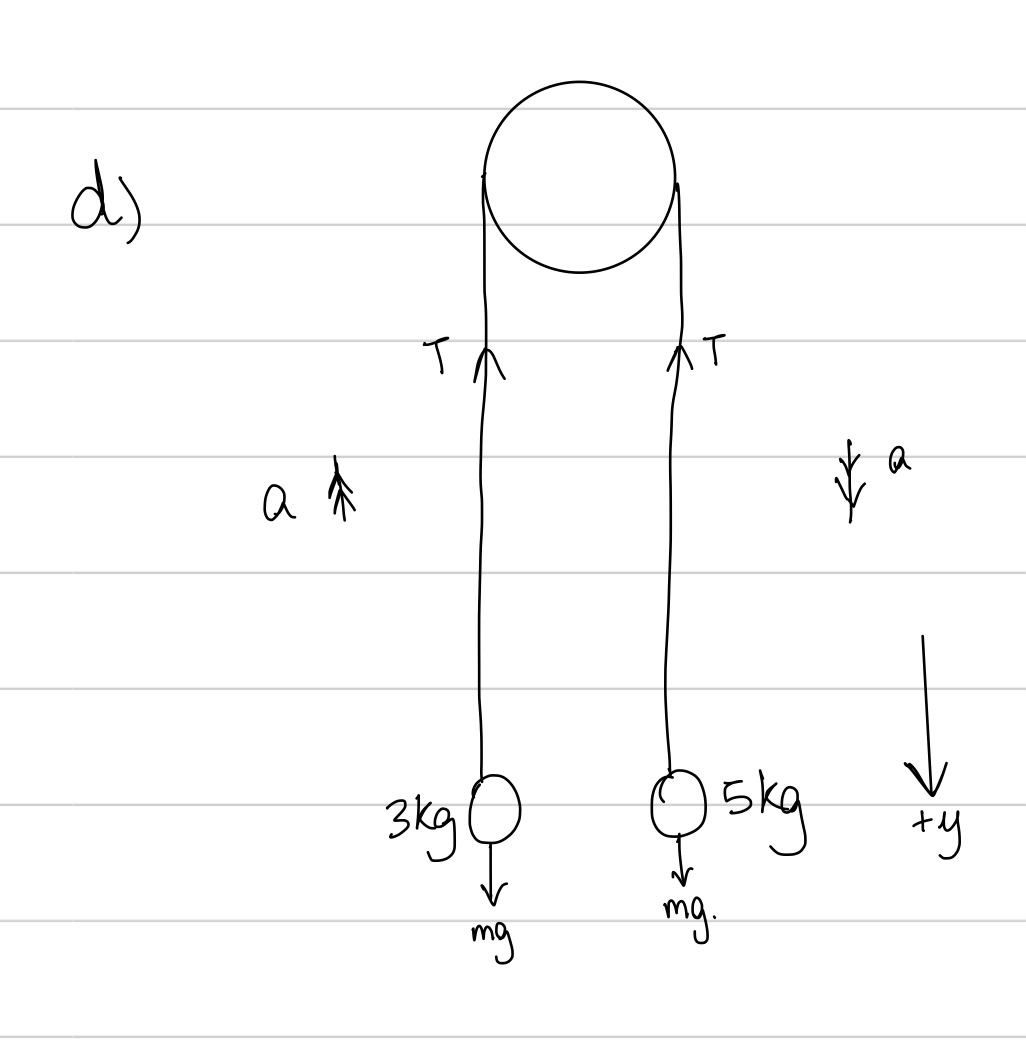
\includegraphics[scale=0.25]{../2015/figures/2015q6-4}
		\caption{\label{2015:q6:fig:Sketch4} Pulley System.}
	\end{center}
\end{figure}	
We are asked to find the acceleration of the system given. This problem is a classic pulley problem and so, we should think about what we know about tension and forces in the context of pulleys.




\textbf{\textit{Simplify and Diagram:}} \\ \\
\begin{figure}[H]
	\begin{center}
		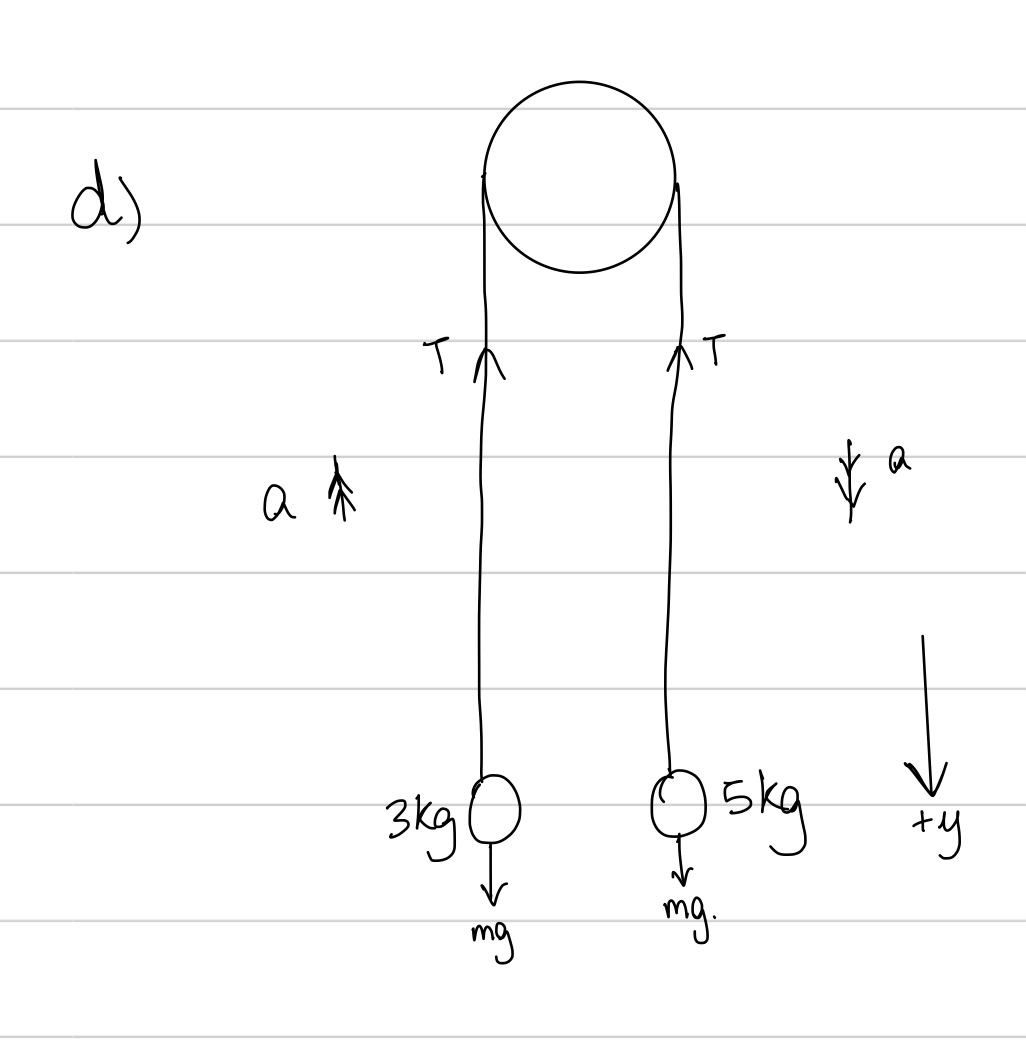
\includegraphics[scale=0.25]{../2015/figures/2015q6-4}
		\caption{\label{2015:q6:fig:Diagram4} All forces on Pulley System.}
	\end{center}
\end{figure}
We will assume that both bodies move in only 1 dimension. We will also assume that the mass of the string is 0 and inextensible. Thus, we know that the speed (and acceleration) of both particles must be the same. Since the pulley is smooth, no energy is lost to friction. We should consider how the forces act on the different weights and motivate our solution from there.




\textbf{\textit{Represent Mathematically:}} \\ \\
Let us first consider the forces on the 5kg mass. From Newton's 2nd Law, we get that,
\begin{align}
	\sum F & = ma \nn \\
	mg - T & = ma \nn \\
	\implies 5g-T & = 5a \,. \label{2015:q6:PulleyEq1}
\end{align}

Let us then consider the forces on the 3kg mass. From Newton's 2nd Law, we get that,
\begin{align}
	\sum F & = ma \nn \\
	 T-mg & = ma \nn \\
	\implies T-3g & = 3a \,. \label{2015:q6:PulleyEq2}
\end{align}




\textbf{\textit{Solve and Evaluate:}} \\ \\
By solving \req{2015:q6:PulleyEq1} and \req{2015:q6:PulleyEq2} simultaneously, we get,
\begin{align}
	\text{(\req{2015:q6:PulleyEq1}+\req{2015:q6:PulleyEq2}):} (5g-T)+[T-3g] & = (5a)+[3a] \nn \\
																	2g & = 8a \nn \\
																	\implies a & = \frac{1}{4}g = 2.5\text{ms}^{-2} \,.
\end{align}




\end{subquestions}